\documentclass[a4paper,14pt]{article}
\usepackage{extsizes}
\usepackage{amsmath}
\usepackage{amssymb}
\everymath{\displaystyle}
\usepackage{geometry}
\usepackage{fancyhdr}
\usepackage{multicol}
\usepackage{graphicx}
\usepackage[brazil]{babel}
\usepackage[shortlabels]{enumitem}
\usepackage{cancel}
\columnsep=2cm
\hoffset=0cm
\textwidth=8cm
\setlength{\columnseprule}{.1pt}
\setlength{\columnsep}{2cm}
\renewcommand{\headrulewidth}{0pt}
\geometry{top=1in, bottom=1in, left=0.7in, right=0.5in}

\pagestyle{fancy}
\fancyhf{}
\fancyfoot[C]{\thepage}

\begin{document}
	
	\noindent\textbf{7FMA157~-~Matemática} 
	
	\begin{center}Interpretando gráficos (Versão estudante)
	\end{center}
	
	
	\noindent\textbf{Nome:} \underline{\hspace{10cm}}
    \noindent\textbf{Data:} \underline{\hspace{4cm}}
	
	%\section*{Questões de Matemática}
	
	\begin{multicols}{2}
		Texto para as questões 1 e 2:
		Considere as contas de luz e de água abaixo. Nelas, é possível verificar o valor a pagar e como calculá-lo em função do consumo de água (m³) e da eletricidade (kWh). Para a conta de luz, o valor a pagar é igual a um fator multiplicado pelo consumo, e para a conta de água, há uma tarifa mínima e diferentes faixas de tarifação.\\\\
		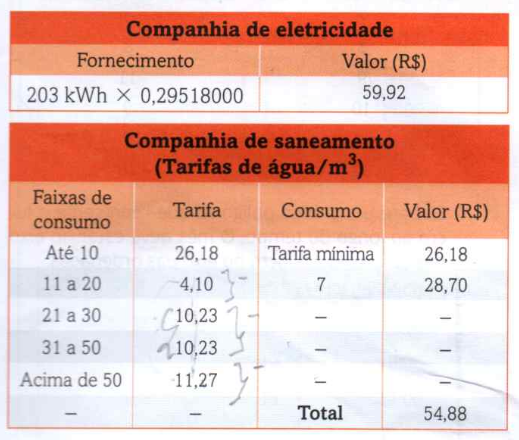
\includegraphics[width=0.45\textwidth]{/home/hogdelta/Documentos/latex/7FMA157_imagens/pg73-1.png}
		\begin{enumerate}
			\item Se no próximo mês o consumo de energia elétrica dobrar, qual o novo valor da conta? \\\\\\\\\\
			\item Dos gráficos a seguir, o que melhor representa o valor da conta de água, de acordo com o consumo, é:
			\begin{enumerate}[a)]
				\item 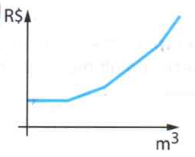
\includegraphics[width=0.30\textwidth]{/home/hogdelta/Documentos/latex/7FMA157_imagens/pg73-2.png}
				\item 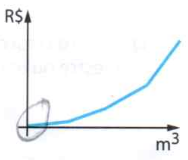
\includegraphics[width=0.30\textwidth]{/home/hogdelta/Documentos/latex/7FMA157_imagens/pg73-3.png}
				\item 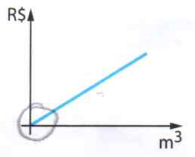
\includegraphics[width=0.30\textwidth]{/home/hogdelta/Documentos/latex/7FMA157_imagens/pg73-4.png}
				\item 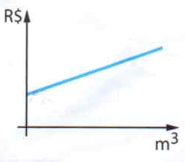
\includegraphics[width=0.30\textwidth]{/home/hogdelta/Documentos/latex/7FMA157_imagens/pg73-5.png}
			\end{enumerate}
			\item A taxa de vacinação contra a gripe em uma cidade nos períodos de 2013 a 2015, e de 2015 a 2017, se deu de forma linear. \\
			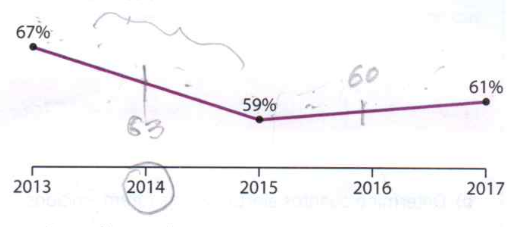
\includegraphics[width=0.45\textwidth]{/home/hogdelta/Documentos/latex/7FMA157_imagens/pg73-6.png} \\
			Desta forma, determine:
			\begin{enumerate}[a)]
				\item A taxa de vacinação em 2014.\\\\\\\\\\
				\item A taxa de vacinação em 2016. \\\\\\\\\\
			\end{enumerate}
			\item Um resumo das médias da temperatura e da umidade relativa do ar de uma cidade, para um período de 15 dias, foi apresentado no gráfico.\\
			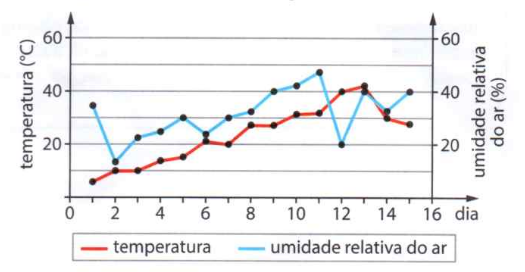
\includegraphics[width=0.45\textwidth]{/home/hogdelta/Documentos/latex/7FMA157_imagens/pg73-7.png} \\
			
			O serviço de meteorologia desta cidade emite relatórios diários com as médias da temperatura e da umidade relativa do ar. De posse dessas informações a prefeitura emite três tipos de alertas para a população:
			
			\begin{itemize}
				\item Alerta cinza: deverá ser emitido sempre que o relatório indicar que a média da temperatura é inferior a 10°C, e a umidade relativa do ar for inferior a 40\%.
				\item Alerta laranja: deverá ser emitido sempre que o relatório indicar que a média da temperatura está entre 30°C e menor que 40°C, e a umidade relativa do ar está abaixo de 30\%.
				\item Alerta vermelho deverá ser emitido sempre que o relatório indicar que a média da temperatura é superior a 40°C, e a humidade relativa do ar for inferior a 25%.
			\end{itemize}
		    \begin{enumerate}[a)]
		    	\item Determine quantos alertas cinzas foram emitidos.\\\\\\\\\\
		    	\item Determine quantos alertas laranja foram emitidos.\\\\\\\\\\
		    	\item Determine quantos alertas vermelhos foram emitidos.\\\\\\\\\\
		    	\item Determine quantos alertas foram emitidos no total.\\\\\\\\\\
		    \end{enumerate}
			\item A seguinte tabela mostra o lucro obtido por uma empresa durante o ano passado.
			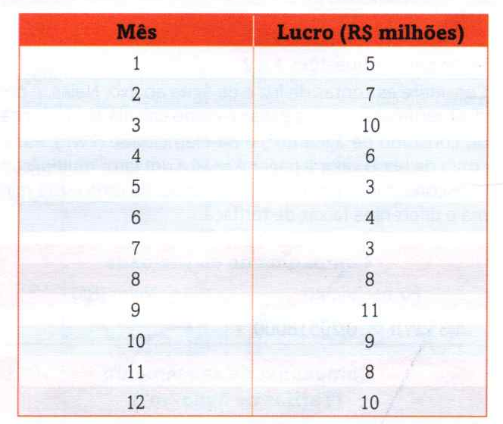
\includegraphics[width=0.45\textwidth]{/home/hogdelta/Documentos/latex/7FMA157_imagens/pg74.png} \\
			\begin{enumerate}[a)]
				\item Elabore um gráfico poligonal que represente o lucro ao longo do tempo. O mês deve estar no eixo das abscissas e o lucro no eixo das ordenadas. \\\\\\\\\\
				\item A partir do gráfico, determine o mês de maior lucro e o maior intervalo de tempo em que houve apenas crescimento no lucro entre meses consecutivos. \\\\\\\\\\
				\item O lucro cresceu mais entre os meses do quarto bimestre ou entre os meses do último? Justifique. \\\\\\\\\\
			\end{enumerate}
		    \item Na semana de 15 a 21 de setembro de 2008, o governo dos Estados Unidos da América divulgou um plano de Socorro às instituições financeiras em crise. O índice da bolsa de valores de São Paulo (Ibovespa) teve forte variação e obteve, no fechamento de cada dia da semana, os seguintes valores: \\
		    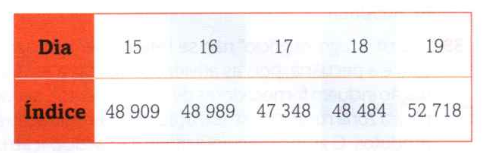
\includegraphics[width=0.45\textwidth]{/home/hogdelta/Documentos/latex/7FMA157_imagens/img1.png} \\
		    O gráfico que representa essa variação é:\\
		    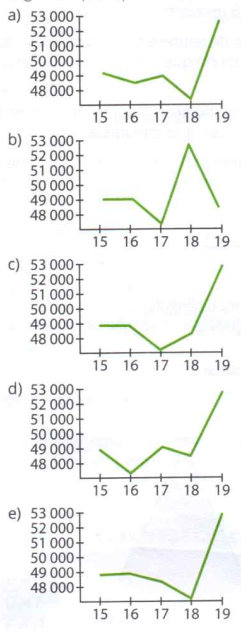
\includegraphics[width=0.45\textwidth]{/home/hogdelta/Documentos/latex/7FMA157_imagens/img2.png} \\
		    
		    \item Qual das afirmações está de acordo com os gráficos a seguir? \\
		    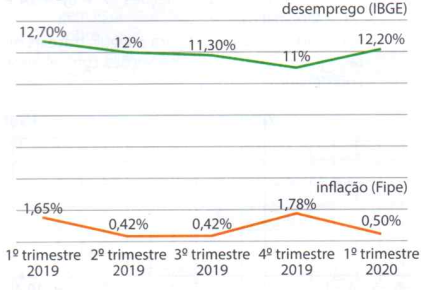
\includegraphics[width=0.45\textwidth]{/home/hogdelta/Documentos/latex/7FMA157_imagens/img3.png} \\
		    \begin{enumerate}[a)]
		    	\item Entre o terceiro e o quarto trimestre de 2019, a taxa de desemprego aumenta.
		    	\item Sempre que a inflação diminui, a taxa de desemprego aumenta.
		    	\item Quando a taxa de desemprego for superior a 12\% a inflação foi menor que 1\%.
		    	\item Sempre que a inflação aumenta, a taxa de desemprego aumenta.
		    	\item A taxa média mensal de desemprego do segundo ao quarto trimestre de 2019 foi igual ou inferior a 12\%.
		    \end{enumerate}
	        \item Observe o gráfico, em que o segmento AB é paralelo ao eixo das abscissas.\\
	        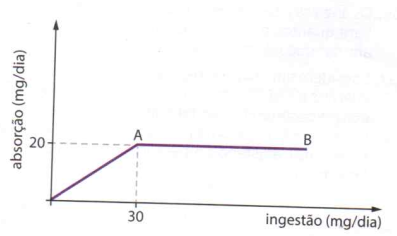
\includegraphics[width=0.45\textwidth]{/home/hogdelta/Documentos/latex/7FMA157_imagens/img4.png} \\
	        Esse gráfico representa a relação entre a ingestão de certo composto, em mg/dia, e sua absorção pelo organismo, também em mg/dia.\\
	        A única alternativa falsa relativa ao gráfico é:\\
	        \begin{enumerate}[a)]
	        	\item Para ingestões acima de 30 mg/dia, quanto maior a ingestão, menor a porcentagem absorvida do composto ingerido.
	        	\item Para ingestões de até 30 mg/dia, absorção é proporcional à quantidade ingerida.
	        	\item Absorção resultante de ingestão de mais de 30 mg/dia é igual a absorção resultante de 30 mg/dia.
	        	\item A razão entre a quantidade de absorvida e a quantidade ingerida é constante.
	        \end{enumerate}
            \item O gráfico abaixo mostra o número de focos de queimadas no Brasil detectados pelo satélite, nos últimos anos, no intervalo de 1 de janeiro até 7 de junho: \\
            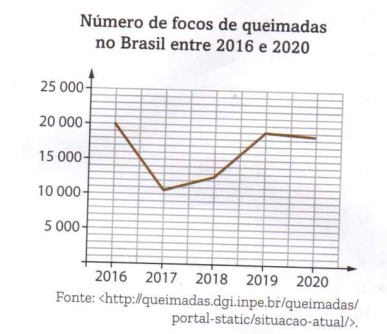
\includegraphics[width=0.45\textwidth]{/home/hogdelta/Documentos/latex/7FMA157_imagens/img5.png} \\
            As informações contidas no gráfico permitem concluir corretamente que, no período considerado:
            \begin{enumerate}[a)]
            	\item O número máximo de focos de queimadas ocorreu em 2019.
            	\item O número aproximado de focos de queimadas no país, em 2020, foi de 17 000.
            	\item A partir de 2018, o número de focos de queimadas no país diminuiu.
            	\item O número mínimo de focos de queimadas ocorreu em 2016.
            	\item De 2018 para 2019 houve um aumento no número de focos de queimadas no país.
            \end{enumerate}
		\end{enumerate}
	$~$ \\ $~$ \\ $~$ \\ $~$ \\ $~$ \\ $~$ \\ $~$ \\ $~$ \\ $~$ \\ $~$ \\ $~$ \\ $~$ \\ $~$ \\ $~$ \\ $~$ \\ $~$ \\ $~$ \\ $~$ \\ $~$ \\ $~$ \\ $~$ \\
    \end{multicols}
	\newpage
	\noindent
	\textbf{Desafio olímpico} \\\\
	A principal atração do parque Gelistone é o gêiser Esguichão. As erupções do gêiser são visíveis de todo o parque, e não duram mais que 3 minutos.
\\
	O gerente do Parque quer maximizar a chance de os visitantes verem de perto uma erupção do esguichando sem, porém deixarem de visitar a loja de lembranças, principal fonte de renda do Parque. Para isso, contratou um estagiário que monitorou o gêiser e anotou os seguintes dados: \\
	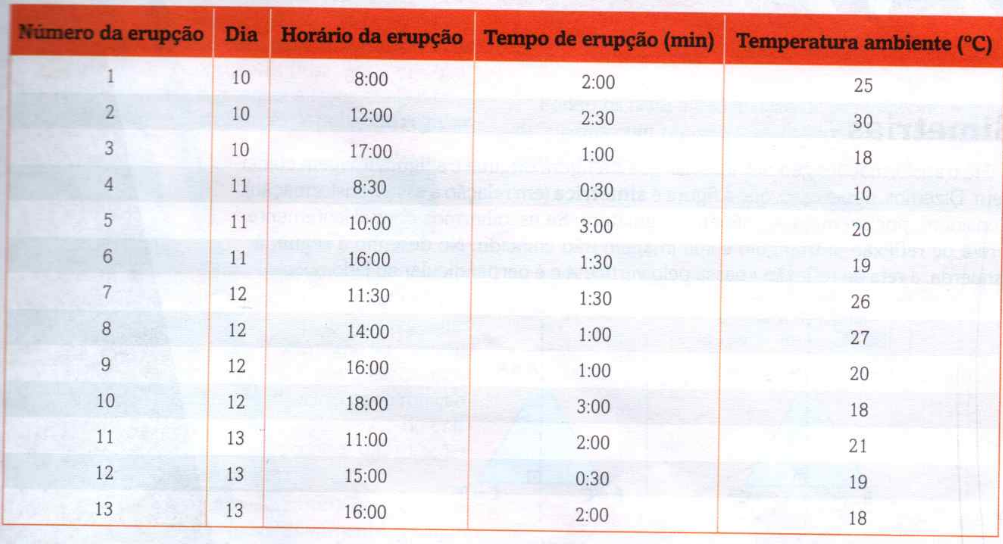
\includegraphics[width=1\textwidth]{/home/hogdelta/Documentos/latex/7FMA157_imagens/pg75.png} \\
	
	\begin{enumerate}[a)]
	\item Faça um gráfico cartesiano, com escala, e marque os pontos (x, y) nos quais x é o tempo da erupção, em minutos, e y é o tempo decorrido entre a erupção correspondente e a próxima erupção, em horas. Você vai ter que descartar a última erupção de cada dia.
	
	
	
	\item Às 7:00 do dia 14, momento em que o parque Abril, o guia do Parque, junto com os visitantes da primeira excursão do dia, viu, ou longe, uma erupção, que durou um minuto e 45 segundos. Utilizando o gráfico que você fez no item (a), estime a que horas a excursão deve chegar nas imediações do Esguichão, para que os visitantes possam ver sua próxima erupção.
	\end{enumerate}
\end{document}









